%\documentclass[twocolumn]{article}
%\usepackage{graphicx}
%\begin{document}
%%% comments begin with a % sign.

\subsubsection{High-energy astrophysics, computational fluid mechanics}
\label{GeoAstro:Bruggen}
\paragraph{Research Team:}
Marcus Br\"uggen (Professor), Elke R\"odiger (Postdoc), Matthias Hoeft
(Postdoc), Thomas  Guimbretiere (PhD student)

%%% give a very short (150 words description of your research area)

My research is concerned with issues in the areas of astrophysical and
computational fluid mechanics, high-energy astrophysics and solar
physics.  Many topics of my research cover a wide range of scales -
from the propagation of waves in the Sun to the dynamics of flows in
galaxies and clusters of galaxies. The macroscopic flows have typical
scales of thousands of kilometers, for instance in stars, to many
thousands of light years in galaxies and clusters of galaxies. These
macroscopic flows are coupled to microscopic processes, such as
viscosity, nuclear flame fronts or radiative processes that take place
on scales of centimetres or lower. It is the major challenge of the
coming years to bridge this huge span in scales which cannot be
resolved by greater computer power alone. Novel algorithms and
numerical techniques have to be invented to model the interactions
between processes on such different scales.


\paragraph{Highlights}

%%% give a short (500 words)description of the research highlights. 1 figure costs 100 words


\noindent Recent observations show a multitude of physical effects
that occur when powerful jets launched by supermassive black holes
interact with the surrounding medium. While these effects are widely
believed to be crucial for the formation of structure in the universe,
they are still poorly understood. Clusters of galaxies are excellent laboratories for studying the
  interaction between active galactic nuclei (AGN) and
  diffuse gas.  Recent observational evidence demonstrates that
  the lives of AGN and their environment are
  closely intertwined. This complex pattern of processes calls for a combined approach of simulations and detailed diagnostics of observations.\\

\noindent Here the main questions are: How is the energy of the jet
dissipated in the intracluster medium (ICM)? How are bubbles, ripples
and waves produced?  What determines the variability of the jet? Is
heating by jets in active galactic nuclei (AGN) universal? How does
feedback operate? What is the kinetic energy output of the AGN? What
is the fate of the ghost bubbles?\\

\noindent Using sophisticated simulations on massively parallel
computers at the National Center for Supercomputing Applications (USA)
and at the Forschungszentrum J\"ulich, we have shown that jets
launched by black holes can prevent the catastrophic cooling in the
centres of galaxies. This project is supported by a recently awarded DFG grant within the
Schwerpunkt 'Witnesses of Cosmic History' supporting a postdoc and a
PhD student.\\

\noindent Moreover, in the past year, we have achieved the following:

\begin{itemize}

\item We have studied the interaction of the jet with its environment, for the first time taking into account the dynamic nature of the cluster gas.  The simulations successfully reproduce the observed morphologies of radio sources in clusters.  We find that cluster inhomogeneities and large-scale flows have significant impact on the morphology of the radio source.

\item With the X-ray telescope XMM-Newton, we have made the deepest observations of the nearest jet from a supermassive black hole and its surroundings. We have identified shock waves and other physical processes in the vicinity of the black hole. We found several new features in M87 related to heating mechanisms of the ICM.

\item When galaxies move through the universe, they experience a head wind. This head wind  can remove the chemical elements that are synthesized in the stars from the gravitational well of the galaxy and disperse it through the universe. The efficiency of this process is unknown, but very important as it influences subsequent structure formation. We produced sophisticated computer models in 3D to determine this efficiency.

\item We have investigated the role of AGN in forming the broad metal abundance peaks observed in cool core clusters. To this end, we carried out numerical simulations that modelled the interplay between metal injection from the central galaxy and the AGN-blown cavities. The resulting distribution patterns were compared to observations.

\item The ICM has a metallicity of about 1/3 solar. However, cooling core clusters,
i.e. clusters with a centrally peaked X-ray brightness, show peaked abundance
profiles. A number of observations indicates that supernovae in the central galaxy
are mainly responsible for the metal enrichment in the central part of
clusters. However, the observed metallicity profiles are much broader than the
light profiles of the central cluster galaxy. Hence, the difference in the
light and the metal distributions are interpreted as the result of transport
processes that have mixed metals into the ICM. We have characterised the AGN-ICM interaction effects by means of deep X-ray observations of nearby clusters, in particular with M87. While it appears to be established that the metals produced by the central galaxy are dispersed into the ICM to form the
broad abundance peaks, it remains unclear what the mechanism is via which the
metals are transported. As one likely mechanism, we studied the effect of AGN-inflated bubbles that rise buoyantly and lift metal-rich gas upwards. We demonstrated that AGN can account for the distribution of metals in clusters of galaxies.

\end{itemize}

% to include a figure, generate a file xxx.pdf and integrate the following lines
\begin{figure}[ht]
  \begin{center}
    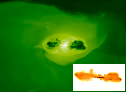
\includegraphics[width=\hsize]{/Bruggen/Brueggen_2006_Fig.png}
    \caption{Snapshots of the gas density in a simulation of a jet in a cluster of
galaxies. One can see how the jet drives shocks into the intracluster
medium. The inset shows the simulated radio emission from this jet.}
    \label{fig:xxx}
  \end{center}
\end{figure}
% to reference it use ``Figure.~\ref{fig:xxx}''; the numbers will be computed automatically.


\paragraph{Organization}
% list the (research) events you have organized, if any,

\begin{enumerate}
\item Tagung des "Rat deutscher Sternwarten", 18. Sep. 2006, IUB
\item Organisation eines DFG Rundgespr\"achs "Astrophysik-Schwerpunkte", 21.-22. Sep. 2006 in Garching
\end{enumerate}

\paragraph{Collaborations}
\begin{enumerate}
\item {\sl University of Colorado}\\ Prof. Markusz Ruszkowski,
  Dr. Eric Hallman,  Prof. Jack Burns
\item {\sl University of Wisconsin}\\ Prof. Sebastian Heinz 
\item {\sl Sterrewacht Leiden}\\ Prof. Joop Schaye and Dr. Claudio
  Dalla Vecchia 
\item {\sl MPI f\"ur Extraterrestrische Physik}\\ Prof. Hans
  B\"ohringer and Dr. Eugene Churazov
\item {\sl Stanford University}\\ Prof. Tom Abel (Stanford)
\item {\sl Los Alamos National Laboratory}\\ Dr. Brian O'Shea (LANL)
\end{enumerate}

\paragraph{Grants}
% list the running grants in 2005, if none have been received, please delete this
% subsection.
\begin{enumerate}

\item Interactions between Active Galactic Nuclei and the Intracluster Medium
(BR 2026/3-1)

\item The CME source region in LOFAR-related simulations (VO 855/2)

\end{enumerate}
\nocite{2006astro.ph.10874S}
\nocite{2006MNRAS.371..609R}
\nocite{2006astro.ph..9831H}
\nocite{2006MNRAS.369..567R}
\nocite{2006astro.ph..6664H}
\nocite{2006AN....327..587B}

% list the publications of 2005 (also accepted and in press), if none have been received, plese delete this
% subsection. Enter the publications into the SES publications database at
% http://kwarc.eecs.iu-bremen.de/ses-pubs/index.php and only reference them here.

%\begin{description}
%  \item[Journals] Nature~\cite{Kohlhase:Nature}, Science~\cite{Kohlhase:Science}
%  \item[Conference Proceedings] CADE~\cite{Kohlhase:CADE1}, ...
%  \item[Books/Collections] \ldots
%\end{description}
%\end{document}

%%% Local Variables:
%%% mode: latex
%%% TeX-master: "RP-EECS"
%%% End:
